% !TEX TS-program = pdflatex
\documentclass[11pt]{article}

% -------------------- Packages --------------------
\usepackage[a4paper,margin=1in]{geometry}
\usepackage{amsmath,amssymb}
\usepackage[T1]{fontenc}
\usepackage{lmodern}
\usepackage{xcolor}
\usepackage{tcolorbox}
\tcbuselibrary{skins,breakable}
\usepackage{enumitem}
\usepackage{hyperref}
\usepackage{tikz}
\usetikzlibrary{calc,arrows.meta}

\pagestyle{empty}

% -------------------- Dark Theme Colors --------------------
\definecolor{bg}{HTML}{000000}
\definecolor{pairbg}{HTML}{121212}
\definecolor{solbg}{HTML}{0A0A0A}
\definecolor{border}{HTML}{2A2A2A}
\definecolor{text}{HTML}{FFFFFF}
\definecolor{muted}{HTML}{C9CDD3}
\definecolor{gold}{HTML}{FFD700}
\definecolor{green}{HTML}{4ADE80}
\definecolor{cyan}{HTML}{38BDF8}

\pagecolor{bg}
\color{text}

\hypersetup{
  colorlinks=true,
  linkcolor=cyan,
  urlcolor=cyan
}

\setlength{\parindent}{0pt}
\setlength{\parskip}{10pt}

% Help LaTeX avoid overfull lines globally
\sloppy
\setlength{\emergencystretch}{3em}

\setlist[itemize]{left=1.4em,itemsep=6pt,topsep=6pt}
\setlist[enumerate]{left=1.6em,itemsep=4pt,topsep=4pt}

% -------------------- tcolorbox Base --------------------
\tcbset{
  enhanced,
  breakable,
  arc=12pt,
  boxrule=0.8pt,
  left=14pt,right=14pt,top=12pt,bottom=12pt
}

\newtcolorbox{QAPair}[1]{%
  colback=pairbg,
  colbacklower=solbg,
  colframe=border,
  coltext=text,
  title=\textcolor{gold}{\bfseries #1},
  fonttitle=\bfseries,
  coltitle=text,
  segmentation style={draw=border, dashed, line width=0.6pt},
  before upper=\raggedright,
  before lower=\raggedright
}

\newtcolorbox{QuickBox}{%
  colback=pairbg,
  colframe=cyan,
  coltext=text,
  fontupper=\color{text}\raggedright,
  borderline north={4pt}{0pt}{cyan},
  arc=14pt,
  boxrule=0.8pt
}

% Helper for step headings
\newcommand{\Step}[1]{\textcolor{muted}{\textbf{Step #1:}}}

% Diagram block (adds breathing space above/below)
\newenvironment{StepDiagram}
  {\par\smallskip\begin{center}\vspace{2pt}}
  {\vspace{2pt}\end{center}\smallskip\par}

% -------------------- TikZ styles (boxed labels = no clashes) --------------------
% IMPORTANT: no blank lines inside \tikzset{...}
\tikzset{
  base/.style={draw=text, line width=0.9pt, line cap=round, line join=round},
  new/.style={draw=cyan, line width=1.2pt, line cap=round, line join=round},
  help/.style={draw=muted, dashed, line width=0.9pt},
  dot/.style={circle, fill=text, inner sep=1.2pt},
  tag/.style={
    font=\small,
    text=text,
    fill=pairbg,
    fill opacity=0.92,
    text opacity=1,
    inner sep=2.2pt,
    rounded corners=4pt
  },
  note/.style={
    font=\small,
    text=muted,
    fill=pairbg,
    fill opacity=0.82,
    text opacity=1,
    inner sep=2.2pt,
    rounded corners=4pt
  }
}

% Safe empty-check helper
\newcommand{\IfEmptyTF}[3]{%
  \if\relax\detokenize{#1}\relax
    #2%
  \else
    #3%
  \fi
}

% Equation callout (safe minipage prevents overflow)
\newcommand{\EqDiagram}[1]{%
\begin{StepDiagram}
\begin{tikzpicture}
\node[
  draw=border,
  rounded corners=10pt,
  inner sep=9pt,
  text=text,
  align=left
]{
  \begin{minipage}{0.86\linewidth}
  \color{text}#1
  \end{minipage}
};
\end{tikzpicture}
\end{StepDiagram}
}

% ------------------------------------------------------------
% Clean Venn: ALL notes go OUTSIDE the rectangle (no overlap)
% #1 left label, #2 right label, #3 bottom note, #4 center label (optional; pass {} if none)
\newcommand{\VennAB}[4]{%
\begin{StepDiagram}
\begin{tikzpicture}[scale=0.95]
  \draw[base, rounded corners=10pt] (-3.3,-2.10) rectangle (3.3,2.10);
  \node[tag] at (-2.9,1.80) {$S$};

  \begin{scope}
    \clip (-3.3,-2.10) rectangle (3.3,2.10);
    \fill[cyan, fill opacity=0.12] (-1.30,0) circle (1.55);
    \fill[gold, fill opacity=0.10] ( 1.30,0) circle (1.55);
  \end{scope}
  \draw[base] (-1.30,0) circle (1.55);
  \draw[base] ( 1.30,0) circle (1.55);

  \node[tag] at (-2.00,1.10) {#1};
  \node[tag] at ( 2.00,1.10) {#2};

  \IfEmptyTF{#4}{}{ \node[tag] at (0,0) {#4}; }

  \node[note] at (0,-2.55) {#3};
\end{tikzpicture}
\end{StepDiagram}
}

% ============================================================
% Quick-formula diagrams (UPDATED to remove top overlaps)

\newcommand{\DiagEquallyLikely}{%
\begin{StepDiagram}
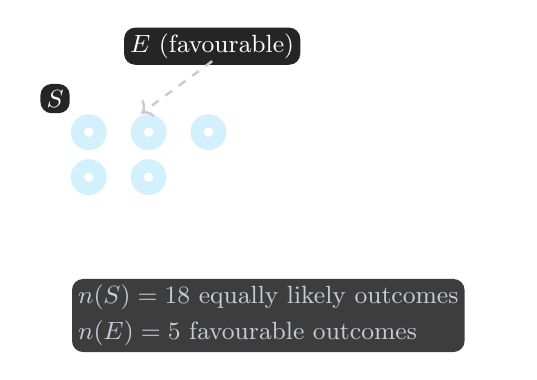
\begin{tikzpicture}[scale=0.95]

  % sample space box
  \draw[base, rounded corners=10pt] (-3.2,-1.35) rectangle (3.2,1.35);
  \node[tag] at (-2.85,1.05) {$S$};

  % 12 equally likely outcomes as dots
  \foreach \x in {-2.4,-1.6,-0.8,0,0.8,1.6}{
    \foreach \y in {-0.6,0,0.6}{
      \node[dot] at (\x,\y) {};
    }
  }

  % highlight 5 favourable dots
  \foreach \p in {(-2.4,0.6),(-1.6,0.6),(-0.8,0.6),(-2.4,0),(-1.6,0)}{
    \fill[cyan, fill opacity=0.22] \p circle (0.24);
    \node[dot] at \p {};
  }

  % move E label ABOVE the box (so it doesn't sit next to S)
  \node[tag] at (-0.75,1.75) {$E$ (favourable)};
  \draw[help,->] (-0.75,1.55) -- (-1.70,0.85);

  % notes OUTSIDE box
  \node[note, align=left] at (0,-1.85)
  {$n(S)=18$ equally likely outcomes\\[2pt]
   $n(E)=5$ favourable outcomes};
\end{tikzpicture}
\end{StepDiagram}
}

\newcommand{\DiagIndependence}{%
\begin{StepDiagram}
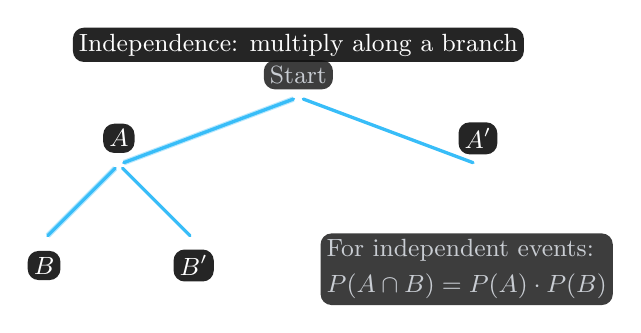
\begin{tikzpicture}[scale=0.95]
  \node[tag] at (0,2.05) {Independence: multiply along a branch};

  \node[dot] (R) at (0,1.35) {};
  \node[note] at (0,1.65) {Start};

  \node[dot] (A)  at (-2.4,0.45) {};
  \node[dot] (Ac) at ( 2.4,0.45) {};
  \draw[new] (R)--(A);
  \draw[new] (R)--(Ac);
  \node[tag] at (-2.4,0.80) {$A$};
  \node[tag] at ( 2.4,0.80) {$A'$};

  \node[dot] (AB)  at (-3.4,-0.55) {};
  \node[dot] (ABc) at (-1.4,-0.55) {};
  \draw[new] (A)--(AB);
  \draw[new] (A)--(ABc);
  \node[tag] at (-3.4,-0.90) {$B$};
  \node[tag] at (-1.4,-0.90) {$B'$};

  \draw[cyan, line width=2.0pt, opacity=0.35] (R)--(A)--(AB);

  \node[note, align=left] at (2.25,-0.95)
  {For independent events:\\[2pt]
   $P(A\cap B)=P(A)\cdot P(B)$};
\end{tikzpicture}
\end{StepDiagram}
}

\newcommand{\DiagAdditionRule}{%
\begin{StepDiagram}
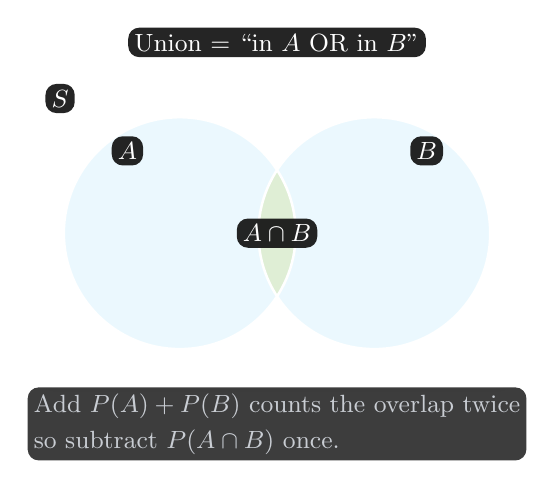
\begin{tikzpicture}[scale=0.95]
  % move the title ABOVE the rectangle (fixes overlap in your screenshot)
  \node[tag] at (0,2.55) {Union = “in $A$ OR in $B$”};

  \draw[base, rounded corners=10pt] (-3.3,-2.10) rectangle (3.3,2.10);
  \node[tag] at (-2.9,1.80) {$S$};

  % Shade union; highlight overlap
  \begin{scope}
    \clip (-3.3,-2.10) rectangle (3.3,2.10);
    \fill[cyan, fill opacity=0.10] (-1.30,0) circle (1.55);
    \fill[cyan, fill opacity=0.10] ( 1.30,0) circle (1.55);
    \begin{scope}
      \clip (-1.30,0) circle (1.55);
      \fill[gold, fill opacity=0.16] (1.30,0) circle (1.55);
    \end{scope}
  \end{scope}

  \draw[base] (-1.30,0) circle (1.55);
  \draw[base] ( 1.30,0) circle (1.55);

  \node[tag] at (-2.00,1.10) {$A$};
  \node[tag] at ( 2.00,1.10) {$B$};
  \node[tag] at (0,0) {$A\cap B$};

  \node[note, align=left] at (0,-2.55)
  {Add $P(A)+P(B)$ counts the overlap twice\\[2pt]
   so subtract $P(A\cap B)$ once.};
\end{tikzpicture}
\end{StepDiagram}
}

\newcommand{\DiagComplement}{%
\begin{StepDiagram}
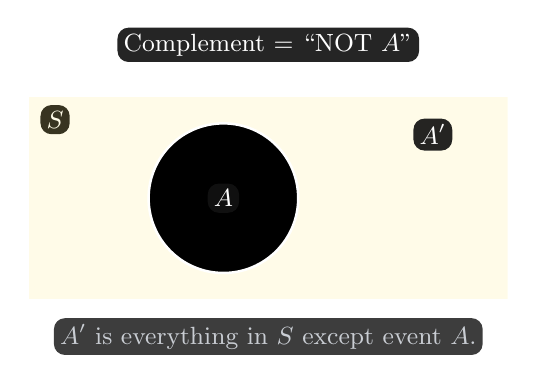
\begin{tikzpicture}[scale=0.95]
  \node[tag] at (0,2.05) {Complement = “NOT $A$”};

  \draw[base, rounded corners=10pt] (-3.2,-1.35) rectangle (3.2,1.35);
  \node[tag] at (-2.85,1.05) {$S$};

  \begin{scope}
    \clip (-3.2,-1.35) rectangle (3.2,1.35);
    \fill[gold, fill opacity=0.09] (-3.2,-1.35) rectangle (3.2,1.35);
    \begin{scope}
      \clip (-0.6,0) circle (1.00);
      \fill[bg] (-3.2,-1.35) rectangle (3.2,1.35);
    \end{scope}
  \end{scope}

  \draw[base] (-0.6,0) circle (1.00);
  \node[tag] at (-0.6,0) {$A$};
  \node[tag] at (2.20,0.85) {$A'$};

  \node[note] at (0,-1.85) {$A'$ is everything in $S$ except event $A$.};
\end{tikzpicture}
\end{StepDiagram}
}

% ============================================================
\begin{document}

\begin{center}
{\LARGE\bfseries \textcolor{gold}{Exercise 12.4 --- Solutions}}\\[-2pt]
\end{center}

% -------------------- Quick formulas + improved diagrams --------------------
\begin{QuickBox}
{\color{cyan}\bfseries Quick formulas (Basic Probability)}\par\medskip

\begin{itemize}
\item \textbf{Equally likely outcomes:} If sample space has $n(S)$ outcomes and event $E$ has $n(E)$ outcomes, then
\[
P(E)=\frac{n(E)}{n(S)}.
\]
\DiagEquallyLikely

\item \textbf{Independent events:} If $A$ and $B$ are independent, then
\[
P(A\cap B)=P(A)\,P(B).
\]
\DiagIndependence

\item \textbf{Addition rule (either $A$ or $B$):}
\[
P(A\cup B)=P(A)+P(B)-P(A\cap B).
\]
\DiagAdditionRule

\item \textbf{Complement:} $P(A')=1-P(A)$.
\DiagComplement
\end{itemize}
\end{QuickBox}

% ============================================================
% Q1
\begin{QAPair}{Question 1}
\textcolor{gold}{\bfseries Question:} Musaab picked a card randomly from a box containing cards bearing numbers $1,2,3$.
He then replaced it and picked another after well shuffling. He found the product of two numbers he got in $2$ trials.
Draw the possibility diagram of this experiment and find probability of getting an even product.
\tcblower
\textcolor{green}{\bfseries Answer:}\par

\Step{1} Since the card is \emph{replaced}, each draw has outcomes $\{1,2,3\}$ and the sample space has
\[
3\times 3 = 9
\quad\text{ordered pairs }(x,y).
\]
\begin{StepDiagram}
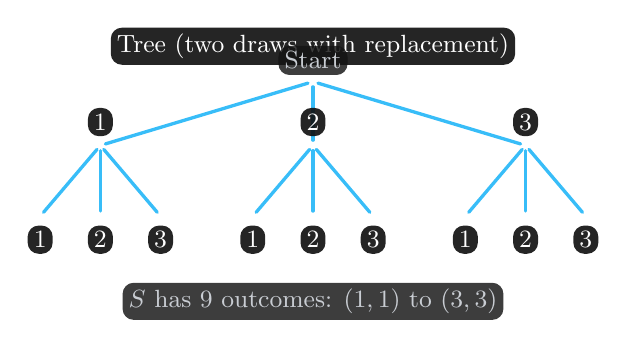
\begin{tikzpicture}[scale=0.90]
  \node[tag] at (0,2.05) {Tree (two draws with replacement)};
  \node[dot] (R) at (0,1.55) {};
  \node[note] at (0,1.85) {Start};

  \foreach \i/\x in {1/-3.0,2/0,3/3.0}{
    \node[dot] (A\i) at (\x,0.65) {};
    \draw[new] (R)--(A\i);
    \node[tag] at (\x,0.98) {\i};

    \foreach \j/\dx in {1/-0.85,2/0,3/0.85}{
      \node[dot] (B\i\j) at (\x+\dx,-0.35) {};
      \draw[new] (A\i)--(B\i\j);
      \node[tag] at (\x+\dx,-0.68) {\j};
    }
  }
  \node[note] at (0,-1.55) {$S$ has $9$ outcomes: $(1,1)$ to $(3,3)$};
\end{tikzpicture}
\end{StepDiagram}

\Step{2} Possibility (product) diagram: write the product $x\cdot y$ for each ordered pair $(x,y)$.
Even products are highlighted.
\begin{StepDiagram}
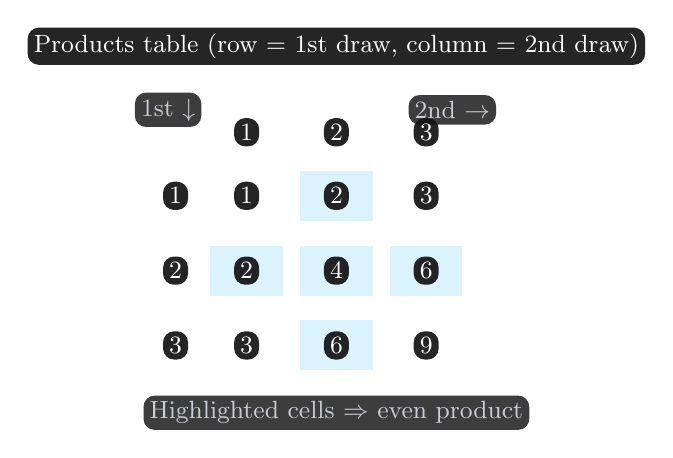
\begin{tikzpicture}[scale=0.95]
  \node[tag] at (0,2.15) {Products table (row = 1st draw, column = 2nd draw)};

  \node[note] at (-2.25,1.30) {1st $\downarrow$};
  \node[note] at ( 1.55,1.30) {2nd $\rightarrow$};

  \foreach \c/\x in {1/-1.2,2/0,3/1.2}{
    \node[tag] at (\x,1.00) {\c};
  }
  \foreach \r/\y in {1/0.15,2/-0.85,3/-1.85}{
    \node[tag] at (-2.15,\y) {\r};
  }

  \foreach \r/\y in {1/0.15,2/-0.85,3/-1.85}{
    \foreach \c/\x in {1/-1.2,2/0,3/1.2}{
      \pgfmathtruncatemacro{\p}{\r*\c}
      \pgfmathtruncatemacro{\m}{mod(\p,2)}
      \ifnum\m=0
        \fill[cyan, fill opacity=0.18] (\x-0.5,\y-0.35) rectangle (\x+0.5,\y+0.35);
      \fi
      \draw[base] (\x-0.5,\y-0.35) rectangle (\x+0.5,\y+0.35);
      \node[tag] at (\x,\y) {\p};
    }
  }
  \node[note] at (0,-2.75) {Highlighted cells $\Rightarrow$ even product};
\end{tikzpicture}
\end{StepDiagram}

\Step{3} A product is even \emph{iff at least one number is $2$}.
So favourable outcomes:
\[
(2,1),(2,2),(2,3),(1,2),(3,2)\ \Rightarrow\ 5 \text{ outcomes.}
\]
\EqDiagram{$\displaystyle P(\text{even product})=\frac{5}{9}$}

\[
\boxed{\frac{5}{9}}
\]
\end{QAPair}

% ============================================================
% Q2
\begin{QAPair}{Question 2}
\textcolor{gold}{\bfseries Question:} Ashas flipped a coin thrice. Draw tree diagram to find the probability of getting three Tails.
\tcblower
\textcolor{green}{\bfseries Answer:}\par

\Step{1} For each flip: $H$ or $T$, each with probability $\tfrac12$.
\begin{StepDiagram}
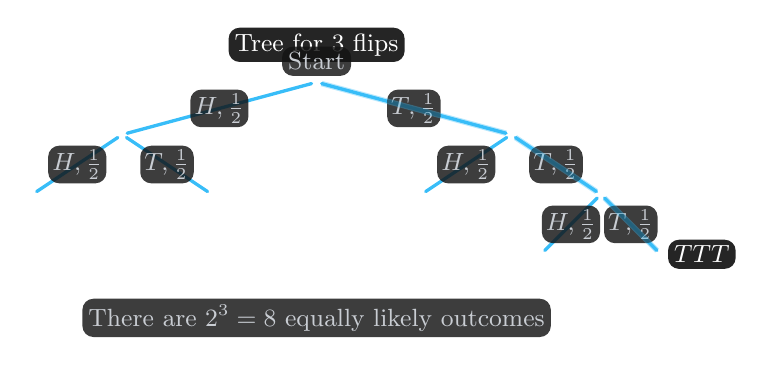
\begin{tikzpicture}[scale=0.95]
  \node[tag] at (0,2.1) {Tree for 3 flips};
  \node[dot] (R) at (0,1.6) {};
  \node[note] at (0,1.88) {Start};

  \node[dot] (A1) at (-2.6,0.9) {};
  \node[dot] (A2) at ( 2.6,0.9) {};
  \draw[new] (R)--(A1) node[midway,note,fill=pairbg,inner sep=1.5pt] {$H,\frac12$};
  \draw[new] (R)--(A2) node[midway,note,fill=pairbg,inner sep=1.5pt] {$T,\frac12$};

  \node[dot] (B11) at (-3.8,0.1) {};
  \node[dot] (B12) at (-1.4,0.1) {};
  \node[dot] (B21) at ( 1.4,0.1) {};
  \node[dot] (B22) at ( 3.8,0.1) {};
  \draw[new] (A1)--(B11) node[midway,note,fill=pairbg,inner sep=1.5pt] {$H,\frac12$};
  \draw[new] (A1)--(B12) node[midway,note,fill=pairbg,inner sep=1.5pt] {$T,\frac12$};
  \draw[new] (A2)--(B21) node[midway,note,fill=pairbg,inner sep=1.5pt] {$H,\frac12$};
  \draw[new] (A2)--(B22) node[midway,note,fill=pairbg,inner sep=1.5pt] {$T,\frac12$};

  \node[dot] (C222) at (4.6,-0.7) {};
  \node[dot] (C221) at (3.0,-0.7) {};
  \draw[new] (B22)--(C221) node[midway,note,fill=pairbg,inner sep=1.5pt] {$H,\frac12$};
  \draw[new] (B22)--(C222) node[midway,note,fill=pairbg,inner sep=1.5pt] {$T,\frac12$};

  \draw[cyan, line width=2pt, opacity=0.35] (R)--(A2)--(B22)--(C222);
  \node[tag] at (5.15,-0.7) {$TTT$};

  \node[note] at (0,-1.55) {There are $2^3=8$ equally likely outcomes};
\end{tikzpicture}
\end{StepDiagram}

\Step{2} Exactly one outcome is $TTT$.
\begin{StepDiagram}
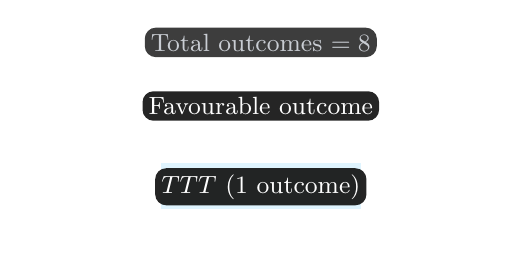
\begin{tikzpicture}[scale=0.95]
  % move the "Total outcomes" note ABOVE the box so it never touches the border
  \node[note] at (0,1.55) {Total outcomes $=8$};

  \draw[base, rounded corners=12pt] (-3.1,-1.05) rectangle (3.1,1.05);

  \node[tag] at (0,0.70) {Favourable outcome};

  \fill[cyan, fill opacity=0.16] (-1.35,-0.05) rectangle (1.35,-0.70);
  \draw[base] (-1.35,-0.05) rectangle (1.35,-0.70);
  \node[tag] at (0,-0.38) {$TTT$ (1 outcome)};
\end{tikzpicture}
\end{StepDiagram}

\Step{3} Hence
\[
P(\text{three tails})=\frac{1}{8}.
\]
\EqDiagram{$\displaystyle P(TTT)=\left(\frac12\right)^3=\frac18$}

\[
\boxed{\frac18}
\]
\end{QAPair}

% ============================================================
% Q3
\begin{QAPair}{Question 3}
\textcolor{gold}{\bfseries Question:} A survey of $100$ students shows that $40$ like pizza, $45$ like burgers.
Draw venn diagram and find probability of students like either pizza or burgers, assuming none like both.
\tcblower
\textcolor{green}{\bfseries Answer:}\par

\Step{1} Since \emph{none like both}, the sets are disjoint.
\begin{StepDiagram}
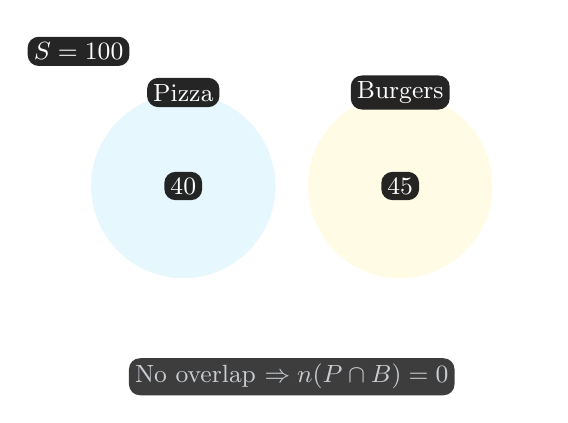
\begin{tikzpicture}[scale=0.95]
  \draw[base, rounded corners=10pt] (-3.3,-2.10) rectangle (3.3,2.10);
  \node[tag] at (-2.85,1.80) {$S=100$};

  \fill[cyan, fill opacity=0.12] (-1.45,0) circle (1.25);
  \fill[gold, fill opacity=0.10] ( 1.45,0) circle (1.25);
  \draw[base] (-1.45,0) circle (1.25);
  \draw[base] ( 1.45,0) circle (1.25);

  \node[tag] at (-1.45,1.25) {Pizza};
  \node[tag] at ( 1.45,1.25) {Burgers};
  \node[tag] at (-1.45,0) {$40$};
  \node[tag] at ( 1.45,0) {$45$};

  \node[note] at (0,-2.55) {No overlap $\Rightarrow n(P\cap B)=0$};
\end{tikzpicture}
\end{StepDiagram}

\Step{2} Students who like \emph{either} pizza or burgers:
\[
n(P\cup B)=40+45=85.
\]
\EqDiagram{$\displaystyle n(P\cup B)=40+45=85$}

\Step{3} Probability:
\[
P(P\cup B)=\frac{85}{100}=0.85.
\]
\EqDiagram{$\displaystyle P(P\cup B)=\frac{85}{100}=0.85$}

\[
\boxed{0.85}
\]
\end{QAPair}

% ============================================================
% Q4
\begin{QAPair}{Question 4}
\textcolor{gold}{\bfseries Question:} What is the probability of a patient testing positive for a disease with either Test A or Test B,
given that $P(A)=0.3$ and $P(B)=0.4$, and the tests are independent?
\tcblower
\textcolor{green}{\bfseries Answer:}\par

\Step{1} Let $A=$ ``positive with Test A'' and $B=$ ``positive with Test B''.
\VennAB{$A$}{$B$}{We want $P(A\cup B)$}{}

\Step{2} Independence gives intersection:
\[
P(A\cap B)=P(A)P(B)=0.3\times 0.4=0.12.
\]
\EqDiagram{$\displaystyle P(A\cap B)=0.3\times 0.4=0.12$}

\Step{3} Use the addition rule:
\[
P(A\cup B)=0.3+0.4-0.12=0.58.
\]
\EqDiagram{$\displaystyle P(A\cup B)=0.58$}

\[
\boxed{0.58}
\]
\end{QAPair}

% ============================================================
% Q5
\begin{QAPair}{Question 5}
\textcolor{gold}{\bfseries Question:} What is the probability of getting either Job A or Job B,
given that $P(A)=0.5$ and $P(B)=0.4$ and the offers are independent?
\tcblower
\textcolor{green}{\bfseries Answer:}\par

\Step{1} Let $A=$ ``get Job A'' and $B=$ ``get Job B''.
\VennAB{$A$}{$B$}{We want $P(A\cup B)$}{}

\Step{2} Since offers are independent:
\[
P(A\cap B)=0.5\times 0.4=0.2.
\]
\EqDiagram{$\displaystyle P(A\cap B)=0.2$}

\Step{3} Addition rule:
\[
P(A\cup B)=0.5+0.4-0.2=0.7.
\]
\EqDiagram{$\displaystyle P(A\cup B)=0.7$}

\[
\boxed{0.7}
\]
\end{QAPair}

% ============================================================
% Q6
\begin{QAPair}{Question 6}
\textcolor{gold}{\bfseries Question:} What is the probability of taking either Volvo bus or Bedford bus to work,
given that $P(V)=\tfrac12$ and $P(B)=\tfrac13$, and the buses are chosen independently?
\tcblower
\textcolor{green}{\bfseries Answer:}\par

\Step{1} Let $V=$ ``take Volvo bus'' and $B=$ ``take Bedford bus''.
\VennAB{$V$}{$B$}{We want $P(V\cup B)$}{}

\Step{2} Independence:
\[
P(V\cap B)=\frac12\cdot\frac13=\frac16.
\]
\EqDiagram{$\displaystyle P(V\cap B)=\frac16$}

\Step{3} Addition rule:
\[
P(V\cup B)=\frac12+\frac13-\frac16
=\frac{3}{6}+\frac{2}{6}-\frac{1}{6}
=\frac{4}{6}=\frac{2}{3}.
\]
\EqDiagram{$\displaystyle P(V\cup B)=\frac{2}{3}$}

\[
\boxed{\frac{2}{3}}
\]
\end{QAPair}

% ============================================================
% Q7
\begin{QAPair}{Question 7}
\textcolor{gold}{\bfseries Question:} What is the probability of either Team Sudaisee or Team Huzaifee winning the championship,
given that $P(S)=\tfrac{12}{27}$ and $P(H)=\tfrac{13}{27}$, and the teams play independently?
\tcblower
\textcolor{green}{\bfseries Answer:}\par

\Step{1} Let $S=$ ``Sudaisee wins'' and $H=$ ``Huzaifee wins''.
\VennAB{$S$}{$H$}{We want $P(S\cup H)$}{}

\Step{2} Independence:
\[
P(S\cap H)=\frac{12}{27}\cdot\frac{13}{27}
=\frac{156}{729}=\frac{52}{243}.
\]
\EqDiagram{$\displaystyle P(S\cap H)=\frac{52}{243}$}

\Step{3} Addition rule:
\[
P(S\cup H)=\frac{12}{27}+\frac{13}{27}-\frac{52}{243}
=\frac{25}{27}-\frac{52}{243}
=\frac{225}{243}-\frac{52}{243}
=\frac{173}{243}.
\]
\EqDiagram{$\displaystyle P(S\cup H)=\frac{173}{243}$}

\[
\boxed{\frac{173}{243}}
\]
\end{QAPair}

% ============================================================
% Q8
\begin{QAPair}{Question 8}
\textcolor{gold}{\bfseries Question:} HJ produces party abayaas. In the products, probability of colour damage is $0.1$
and probability of bad stitching is $0.2$. Find the probability of a product having either colour damage or bad stitching.
\tcblower
\textcolor{green}{\bfseries Answer:}\par

\Step{1} Let $C=$ ``colour damage'' and $S=$ ``bad stitching''.
\VennAB{$C$}{$S$}{We want $P(C\cup S)$}{}

\Step{2} (Standard assumption in such questions) treat defects as independent:
\[
P(C\cap S)=0.1\times 0.2=0.02.
\]
\EqDiagram{$\displaystyle P(C\cap S)=0.02$}

\Step{3} Addition rule:
\[
P(C\cup S)=0.1+0.2-0.02=0.28.
\]
\EqDiagram{$\displaystyle P(C\cup S)=0.28$}

\[
\boxed{0.28}
\]
\end{QAPair}

% ============================================================
% Q9
\begin{QAPair}{Question 9}
\textcolor{gold}{\bfseries Question:} Fakeha is tested for a disease with Test A and Test B and
$P(A)=0.9$, $P(B)=0.7$. Find the probability of testing positive with \emph{both} Test A and Test B, when the tests are independent.
\tcblower
\textcolor{green}{\bfseries Answer:}\par

\Step{1} Model as a two-step tree (A then B).
\begin{StepDiagram}
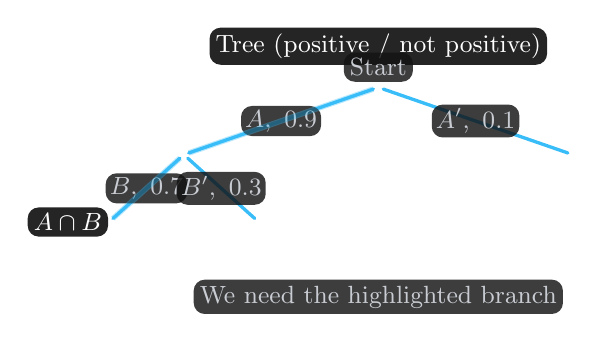
\begin{tikzpicture}[scale=0.95]
  \node[tag] at (0,2.1) {Tree (positive / not positive)};
  \node[dot] (R) at (0,1.55) {};
  \node[note] at (0,1.82) {Start};

  \node[dot] (Apos) at (-2.6,0.65) {};
  \node[dot] (Aneg) at ( 2.6,0.65) {};
  \draw[new] (R)--(Apos) node[midway,note,fill=pairbg,inner sep=1.5pt] {$A,\ 0.9$};
  \draw[new] (R)--(Aneg) node[midway,note,fill=pairbg,inner sep=1.5pt] {$A',\ 0.1$};

  \node[dot] (Both) at (-3.6,-0.25) {};
  \node[dot] (Aonly) at (-1.6,-0.25) {};
  \draw[new] (Apos)--(Both) node[midway,note,fill=pairbg,inner sep=1.5pt] {$B,\ 0.7$};
  \draw[new] (Apos)--(Aonly) node[midway,note,fill=pairbg,inner sep=1.5pt] {$B',\ 0.3$};

  \draw[cyan, line width=2pt, opacity=0.35] (R)--(Apos)--(Both);
  \node[tag] at (-4.15,-0.25) {$A\cap B$};
  \node[note] at (0,-1.25) {We need the highlighted branch};
\end{tikzpicture}
\end{StepDiagram}

\Step{2} Independence:
\[
P(A\cap B)=P(A)P(B)=0.9\times 0.7.
\]
\EqDiagram{$\displaystyle P(A\cap B)=0.9\times 0.7$}

\Step{3} Compute:
\[
0.9\times 0.7=0.63.
\]
\EqDiagram{$\displaystyle P(A\cap B)=0.63$}

\[
\boxed{0.63}
\]
\end{QAPair}

% ============================================================
% Q10
\begin{QAPair}{Question 10}
\textcolor{gold}{\bfseries Question:} Cocobakes produces festive cakes. The quality control department performs 2 quality checks
A and B on an item. Find the probability of a product passing both Quality Control Test A and Test B,
given that $P(A)=0.9$ and $P(B)=0.8$, and the tests are independent.
\tcblower
\textcolor{green}{\bfseries Answer:}\par

\Step{1} Passing both tests means event $A\cap B$.
\VennAB{$A$ (pass A)}{$B$ (pass B)}{We want $P(A\cap B)$}{$A\cap B$}

\Step{2} Independence:
\[
P(A\cap B)=P(A)P(B)=0.9\times 0.8.
\]
\EqDiagram{$\displaystyle P(A\cap B)=0.9\times 0.8$}

\Step{3} Compute:
\[
0.9\times 0.8=0.72.
\]
\EqDiagram{$\displaystyle P(\text{pass both})=0.72$}

\[
\boxed{0.72}
\]
\end{QAPair}

\end{document}
